\begin{figure}[htbp]
  %\null\hfill
  \subfloat[SCT Bayesian linear regressor.]{
	  \includegraphics[width=.48\columnwidth]{images/069sctbayesianlinearregressor}
	  \label{fig:069sctbayesianlinearregressor}
  }
  \quad
    \subfloat[SCT Gaussian non linear regressor.]{
	  \includegraphics[width=.48\columnwidth]{images/070sctgaussiannonlinearregressor}
	  \label{fig:070sctgaussiannonlinearregressor}
  }
  \\
 % \hfill
  \subfloat[SCT ANN non linear regression.]{
	  \includegraphics[width=.48\columnwidth]{images/071annnonlinearregressor}
	  \label{fig:071annnonlinearregressor}
  }
  \quad
    \subfloat[AoR Bayesian linear regressor.]{
	  \includegraphics[width=.48\columnwidth]{images/072aorbayesianlinearregression}
	  \label{fig:072aorbayesianlinearregression}  }
  \\
    \subfloat[AoR Gaussian non linear regressor.]{
	  \includegraphics[width=.48\columnwidth]{images/073aorgaussiannonlinearregression}
	  \label{fig:073aorgaussiannonlinearregression}
  }
  \quad
 % \hfill
  \subfloat[AoR ANN non linear regression.]{
	  \includegraphics[width=.48\columnwidth]{images/074aorannnonlinearegression}
	  \label{fig:074aorannnonlinearegression}
  }
 % \hfill\null
  \caption{Regressions.
  \change{Decide if to put AoR regression images. In case improve them.}
  }
  \label{fig:077regressions}
\end{figure}

% \begin{figure}%[!h] 
% \centering 
% 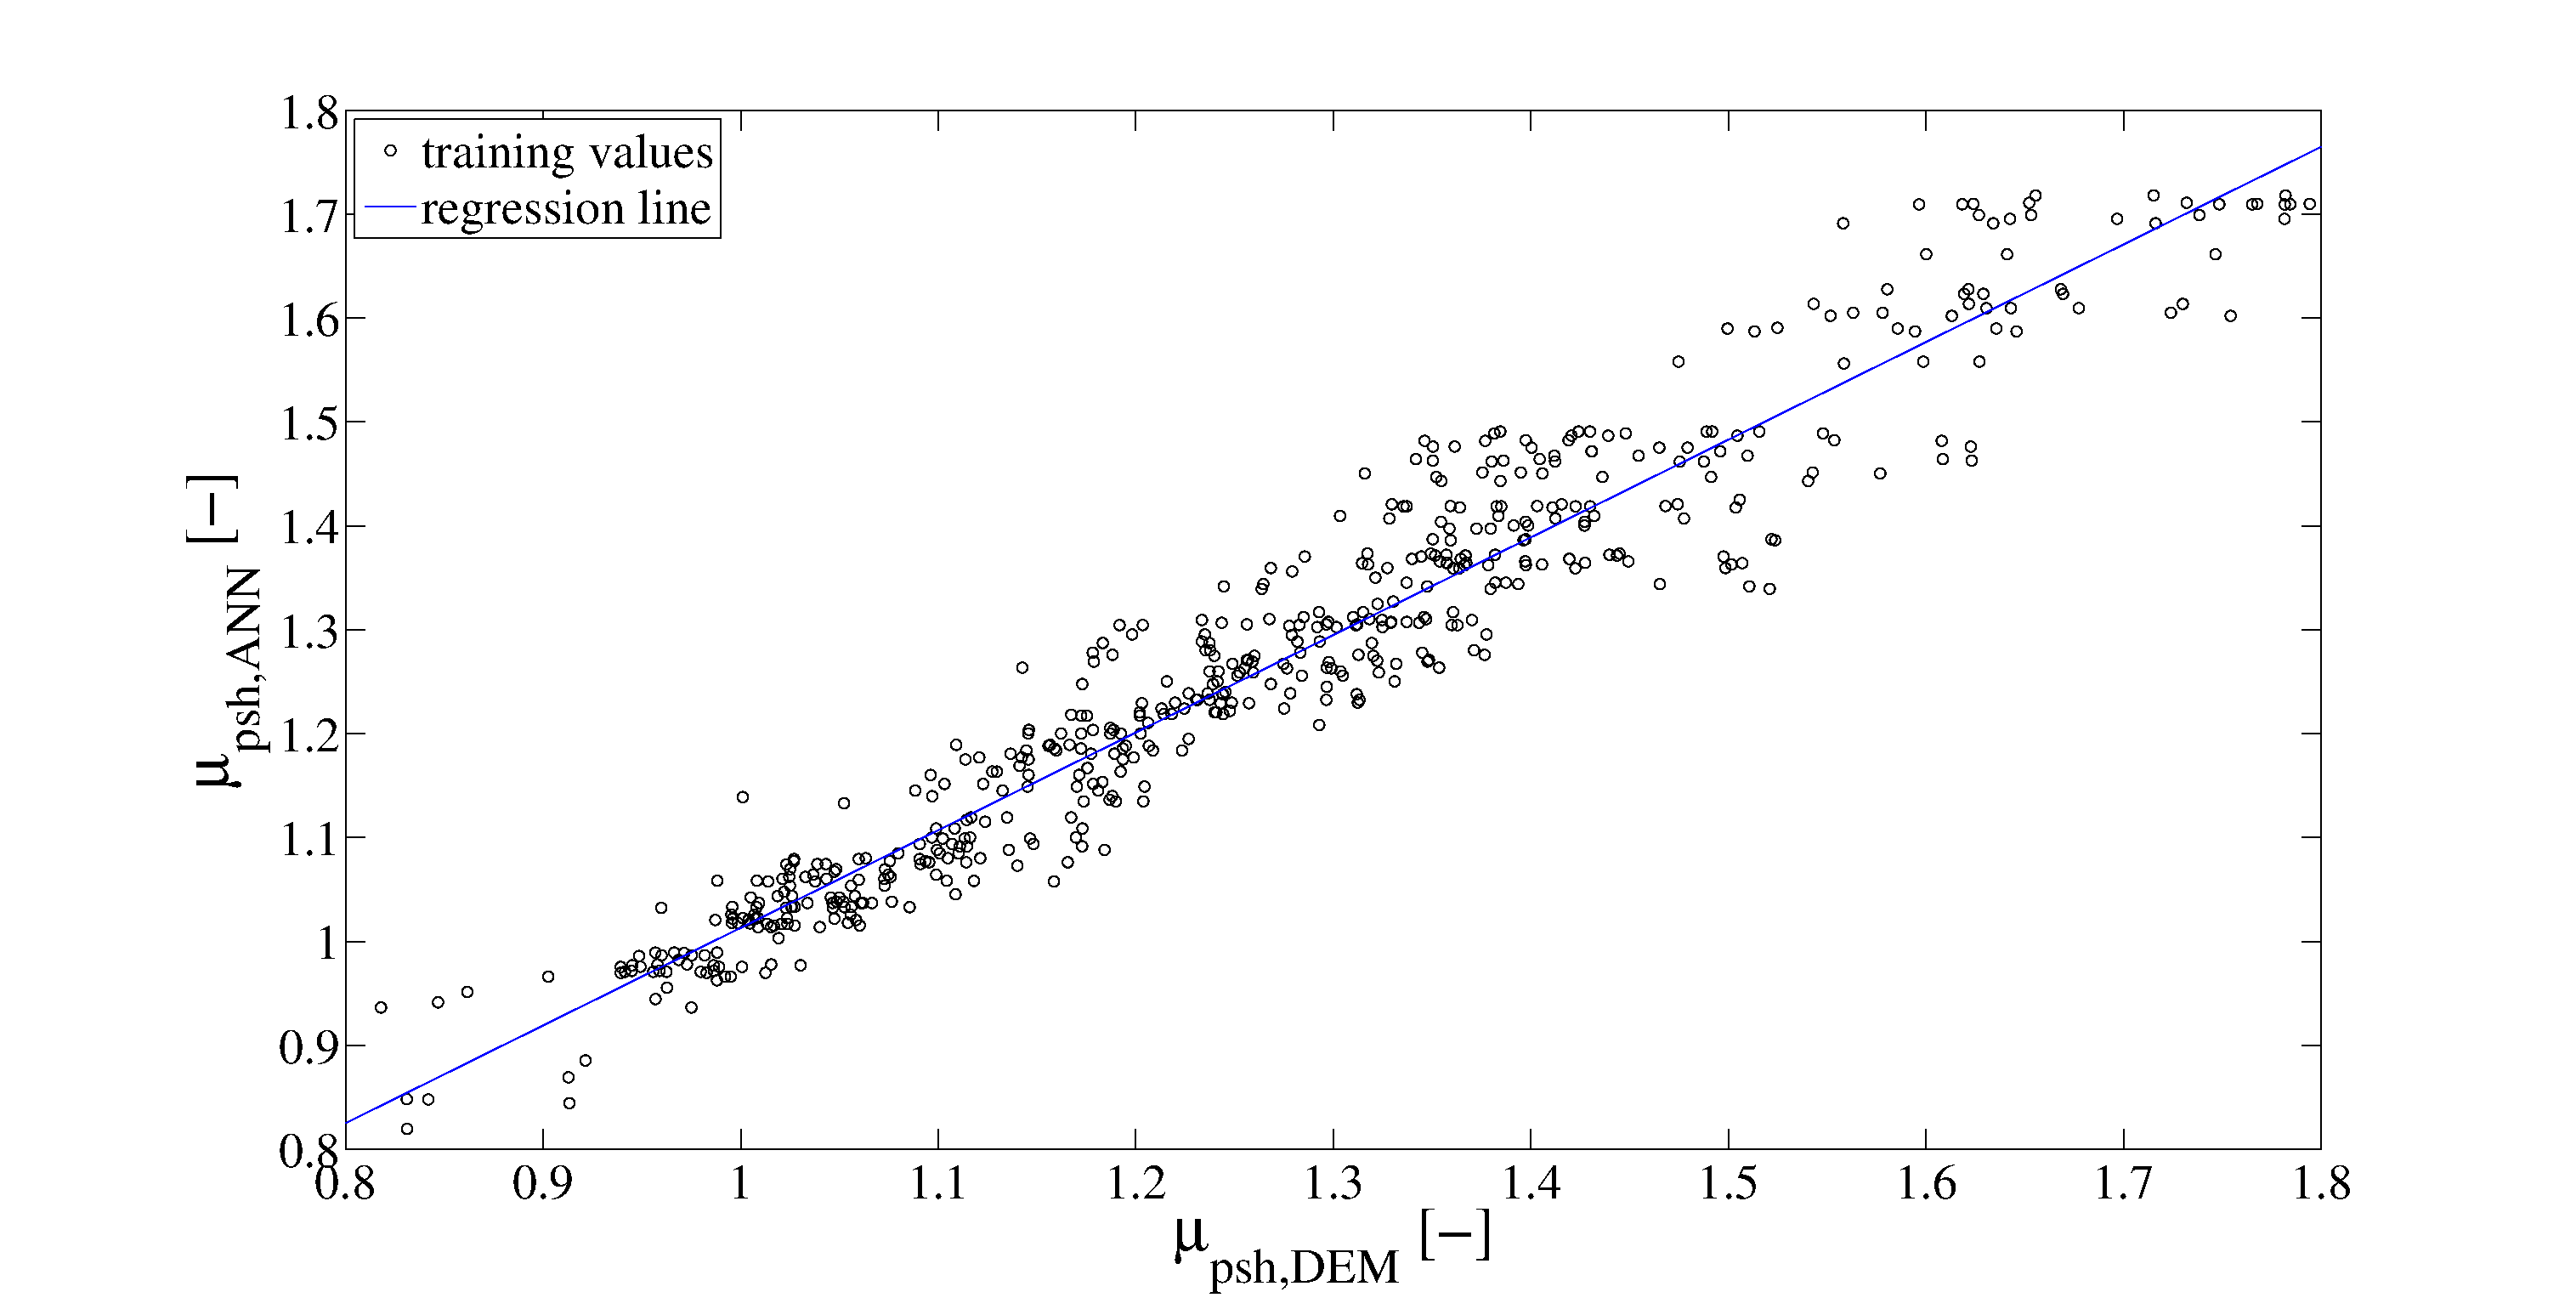
\includegraphics[width=.80\columnwidth]{images/022regression.eps}
% %[width=.48\textwidth]
% \caption[Comparison between prediction of the trained ANN and full DEM
% simulation]{Comparison between prediction of the trained Artificial Neural
% Network (\acs{ANN}) and 546 
% \wrong{write down all the simulations performed at the end.}
% full DEM simulations of the coefficient of pre-shear
% (\acs{mupsh}).}
% \label{fig:022regression} 
% \end{figure}